\documentclass[11pt,a4paper]{scrartcl}

\usepackage[T1]{fontenc}
\usepackage[utf8]{inputenc}
\usepackage[english]{babel}
\usepackage{microtype}
\usepackage{amsmath,amssymb,mathtools}
\usepackage{booktabs}
\usepackage{enumitem}
\usepackage{xcolor}
\usepackage[autostyle]{csquotes}
\usepackage{tikz}
\usetikzlibrary{arrows.meta,positioning,calc}
\usepackage{xurl}
\usepackage[hidelinks]{hyperref}
\usepackage[backend=biber,style=numeric,sorting=nyt,maxbibnames=99]{biblatex}
\addbibresource{references.bib}
\AtBeginBibliography{\sloppy}

\newcommand{\vlinehaul}{v_{\mathrm R}}
\newcommand{\vstation}{v_{\mathrm S}}
\newcommand{\hlinehaul}{h_{\mathrm R}}
\newcommand{\hmerge}{h_{\mathrm M}}
\newcommand{\hservice}{h_{\mathrm S}}

\title{Derivation and Provenance of the Artificial Ropeway Topology Parameters}
\author{Felix Fricke}
\date{Working note, 17 August 2026}

\begin{document}
\maketitle

\begin{abstract}
This note derives the physical and logical parameters of two small artificial
ropeway topologies used to evaluate demand-aware skip-stop operation.  Its
central methodological rule is that line, merge, and station headways are
different quantities.  In particular, a conventional carrier pitch such as
60~m is not interpreted as a safety-only minimum on a future skip-stop line.
Every numerical value is classified as a normative limit, an empirical design
reference, a geometric derivation, or an experimental assumption.  This keeps
the experiments reproducible without claiming engineering certification for a
not-yet-built bypass and merge mechanism.
\end{abstract}

\tableofcontents

\section{Scope and evidence classes}

Urban monocable detachable gondolas commonly combine a fast line movement
with slow, detached movement through stations.  Reviews establish the
technology as an urban public-transport mode, but also show considerable
variation between installations \cite{alshalalfah2012,ppiaf2020}.  No single
published installation therefore determines all parameters of the artificial
experiment.

We use four evidence classes:
\begin{enumerate}[label=\textbf{E\arabic*.},leftmargin=*]
  \item \textbf{Normative limit:} a value or design obligation stated by a
    regulation or technical standard.
  \item \textbf{Empirical reference:} a value reported for an existing or
    manufacturer-coordinated design.
  \item \textbf{Derived parameter:} a value computed from explicitly stated
    geometry or kinematics.
  \item \textbf{Experimental assumption:} a controlled factor selected to
    isolate a mechanism; it is not presented as a certified design value.
\end{enumerate}

European regulation requires vehicle speed, minimum vehicle distance,
acceleration, and braking performance to ensure passenger safety, but it does
not prescribe one universal gondola headway \cite{eu2016ropeways}.  Likewise,
EN~12929-1 requires the smallest interval and carrier pitch of a detachable
unidirectional ropeway to account for line loading, loading and unloading,
acceleration and deceleration, and passage through stations
\cite[Sec.~9.3]{en12929}.  Consequently, a pure safety headway and a complete
certified installation pitch must not be conflated.

\section{Artificial topologies}

\subsection{Six-station line}

The bidirectional line is
\[
T_0 \leftrightarrow S_1 \leftrightarrow S_2 \leftrightarrow
S_3 \leftrightarrow S_4 \leftrightarrow T_5.
\]
The terminals $T_0,T_5$ are mandatory and include turnaround movements.  The
four intermediate stations have a service route and a bypass route in each
direction.  Six stations are not a literature-derived optimum.  They are the
smallest convenient experimental assumption that provides two mandatory
terminal bottlenecks and four intermediate resources from which materially
different stop patterns can be formed.

\subsection{Bidirectional six-station ring}

The ring consists of the cycle $(S_0,S_1,\ldots,S_5,S_0)$ in both clockwise
and counter-clockwise directions.  The two directions use distinct directional
rope resources.  Every station has service and bypass routes; cabins remain in
one direction in the baseline experiment.  This topology removes mandatory
terminal processing and therefore separates the effect of avoidable station
resources from the terminal bottleneck of the line.

\begin{figure}[ht]
  \centering
  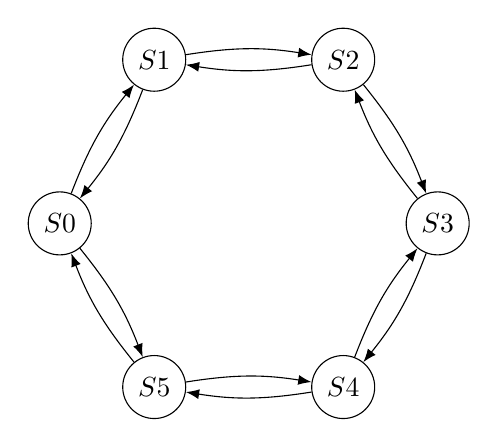
\begin{tikzpicture}[
    station/.style={circle,draw,minimum size=8mm,inner sep=1pt},
    >=Latex]
    \foreach \name/\angle in {S0/180,S1/120,S2/60,S3/0,S4/-60,S5/-120} {
      \node[station] (\name) at (\angle:2.4cm) {$\name$};
    }
    \foreach \a/\b in {S0/S1,S1/S2,S2/S3,S3/S4,S4/S5,S5/S0} {
      \draw[->,bend left=9] (\a) to (\b);
      \draw[->,bend left=9] (\b) to (\a);
    }
  \end{tikzpicture}
  \caption{Artificial bidirectional ring.  Opposite arrows represent distinct
  directional rope resources rather than overtaking on one rope.}
\end{figure}

\section{Spatial and operating parameters}

\subsection{Interstation distance}

There is no universal urban-ropeway station spacing: alignments depend on
topography, property, access, and integration with the surrounding transit
network \cite{alshalalfah2012,ppiaf2020}.  The baseline uses equal adjacent
distances
\[
L_{\mathrm{seg}}=300\ \mathrm m
\]
as an experimental assumption.  At the selected line speed this produces a
50~s interstation line-haul time, long enough for station skipping to have a
visible but not overwhelming travel-time effect:
\[
t_{\mathrm{seg}}=\frac{L_{\mathrm{seg}}}{\vlinehaul}
=\frac{300}{6}=50\ \mathrm s.
\]
A possible robustness analysis with alternative segment lengths is deferred
until after the single reference case has been evaluated.  This is more
defensible than labeling 300~m a typical or mandatory real-world value.

\subsection{Line and station speeds}

For closed, detachable monocable carriers, EN~12929-1 gives 6~m/s on the line
and at most 0.5~m/s in loading and unloading areas
\cite[Sec.~9.2.5]{en12929}.  The French supervisory authority reports the same
limits and cabin capacities of up to ten seated or sixteen standing passengers
\cite{strmtgGondola}.  We therefore set
\[
\vlinehaul=6.0\ \mathrm{m/s}.
\]
The service-platform speed is set to
\[
\vstation=0.3\ \mathrm{m/s},
\]
which is below the normative maximum and equals the manufacturer-coordinated
Regensburg simulation assumption \cite{haimerl2022}.  It is an empirical
reference, not a universal boarding-speed requirement.  The first experiment
keeps this value fixed rather than treating station speed as a sensitivity
factor.

\subsection{Cabin capacity and logical station geometry}

The baseline capacity is ten passengers, supported both by the French system
description and by the Regensburg study \cite{strmtgGondola,haimerl2022}.
Te\v{z}ak et al. use a 3.0~m vehicle length and a 0.5~m minimum in-station
clearance to derive a 3.5~m station pitch \cite{tezak2016}.  We adopt this
published calculation as the service-channel reference.  The remaining route
lengths are experimental geometry compatible with the current software
abstraction:
\begin{center}
\begin{tabular}{@{}lll@{}}
\toprule
Quantity & Baseline & Evidence class \\
\midrule
Cabin capacity & 10 passengers & empirical reference \\
Cabin length $L_C$ & 3.0 m & published model reference \\
Service platform length & 10 m & experimental abstraction \\
Bypass path length & 20 m & experimental abstraction \\
Fast approach/departure connector & 5 m each & experimental abstraction \\
Brake/acceleration connector & 3 m each & timing abstraction \\
Compressed station clearance $c_S$ & 0.5 m & published model reference \\
\bottomrule
\end{tabular}
\end{center}
These lengths do not constitute a civil-engineering station layout.  In
particular, a 3~m braking connector is not claimed to be sufficient for a
6~m/s-to-0.3~m/s physical deceleration.  A later engineering layout may replace
these logical route lengths while preserving the resource model.

Multiple platforms and independently stopped intermediate-station vehicles
have been proposed specifically to increase urban cable-car capacity
\cite{tezak2016}.  That work motivates the bypass experiment and the station
pitch, but does not by itself certify the compact bypass geometry above.

\section{Safety-based separation of headways}

\subsection{Why one spacing parameter is invalid}

The current software parameter \texttt{required\_cabin\_spacing\_m} is used to
derive both rope and station durations.  This is unsuitable for the proposed
experiments.  Computing
\[
d_{\mathrm R}=\vlinehaul\frac{L_C+c_S}{\vstation}
\]
would transfer the slow service-platform pitch to the line.  It would assume
away precisely the possible capacity advantage under investigation.

The model instead requires three independent quantities:
\begin{align*}
\hlinehaul &\quad\text{for attached carriers on a common rope},\\
\hmerge    &\quad\text{for merge and attachment},\\
\hservice  &\quad\text{for service-platform processing}.
\end{align*}

\subsection{Attached carriers on the line}

For two correctly attached carriers on the same moving rope, their attachment
points have a fixed relative distance.  A common drive stop does not create the
rear-end closure familiar from independently driven road or rail vehicles.
The safety-only longitudinal separation is therefore primarily a swept-envelope
condition under carrier sway, while line loading is treated as a separately
dimensioned engineering constraint.

EN~12929-1 and the French RM2 guidance require a longitudinal sway angle of at
least
\[
\theta_R=0.34\ \mathrm{rad}
\]
on the line and in stations unless a justified reduction applies
\cite[Sec.~6.3.5]{en12929,strmtgRM2}.  Let $\ell_H$ denote the vertical distance
from the attachment point to the cabin reference point and let $c_R$ be the
free distance that remains between two worst-case longitudinal movement
envelopes.  A simplified symmetric-envelope approximation gives
\begin{equation}
d_{\mathrm R}^{\mathrm{swing}}
  \ge L_C+2\ell_H\sin(\theta_R)+c_R.
\label{eq:swing-spacing}
\end{equation}
The corresponding headway is
\begin{equation}
\hlinehaul^{\mathrm{swing}}
  =\frac{d_{\mathrm R}^{\mathrm{swing}}}{\vlinehaul}.
\label{eq:swing-headway}
\end{equation}
The standard fixes neither $\ell_H$ nor $c_R$: $\ell_H$ is carrier-specific and
$c_R$ is a design safety allowance.  The French guidance uses an additional
0.3~m envelope margin in specified clearance cases \cite{strmtgRM2}; this is
not a general adjacent-carrier requirement.  The initial reference case uses
$c_R=0.5$~m as an explicit experimental assumption and requires a manufacturer
value for $\ell_H$ before any engineering interpretation.  For illustration,
$L_C=3$~m, $\ell_H=3$~m, $c_R=0.5$~m, and
$\vlinehaul=6$~m/s yield
\[
d_{\mathrm R}^{\mathrm{swing}}\approx5.5\ \mathrm m,
\qquad
\hlinehaul^{\mathrm{swing}}\approx0.92\ \mathrm s.
\]
Neither the illustrative 3~m suspension length nor the resulting 0.92~s is a
literature-backed operating value.  The calculation demonstrates only that the
familiar 60~m pitch cannot be justified by adjacent-cabin sway alone.  Exact
carrier CAD envelopes may replace Eq.~\eqref{eq:swing-spacing} by
\[
d_{\mathrm R}^{\mathrm{swing}}=e_R^-+e_R^++c_R,
\]
where $e_R^-,e_R^+$ are the maximum fore and aft projections.  Grip behaviour,
tower passage, control tolerances, and a safety assessment remain necessary.

Accordingly, the complete design headway is conceptually
\begin{equation}
\hlinehaul=\max\{h_R^{\mathrm{swing}},h_R^{\mathrm{tower}},
h_R^{\mathrm{grip}},h_R^{\mathrm{loading}},h_R^{\mathrm{control}},\ldots\}.
\label{eq:complete-rope-headway}
\end{equation}
The artificial short-headway case makes the explicit experimental hypothesis
that the installation is dimensioned so that the geometric term dominates.
Thus it sets $h_R=h_R^{\mathrm{swing}}=0.92$~s conditionally; it does not claim
that 0.92~s is certified for a present installation.

Grip failure is a separate safety function.  A larger ordinary headway cannot
make complete loss of attachment safe.  Standards instead require monitoring
of detachable carriers and safe handling of improperly attached carriers near
station exits \cite[Secs.~5.4.2 and 9.3.2]{en12929}.  The optimization must not
silently substitute a spacing constraint for those engineering protections.

\subsection{Merge safety and attachment resources}

At a service/bypass merge, collision separation, the attachment mechanism, and
the availability of a free rope slot are distinct resources.  Let
$\tau_M^{\mathrm{stop}}$ bound the time from the earliest hazardous condition
until the relevant following carrier or its conveyor is safely stationary:
\begin{equation}
\tau_M^{\mathrm{stop}}
=\tau^{\mathrm{detect}}+\tau^{\mathrm{logic}}
 +\tau^{\mathrm{communication}}+\tau^{\mathrm{actuation}}
 +\tau^{\mathrm{braking}}.
\label{eq:merge-stop-time}
\end{equation}
The bound includes sensor placement and all communication delays; it does not
start only when a downstream sensor finally reports the fault.  Existing
stations monitor carrier presence, speed, clamping, and collision hazards
\cite{stationSafetyDevices2017}, but the end-to-end guarantee remains
installation-specific \cite[Sec.~9.3.2]{en12929}.

The carriers must additionally remain geometrically separated while they may
swing.  For a tangential service/bypass merge, let $v_M$ be the upper speed at
the common conflict location, $\theta_M^{\mathrm{emergency}}$ the emergency
longitudinal sway angle, $\ell_H$ the suspension length, and $c_M$ an additional
clearance.  The conservative swept-envelope distance and its time equivalent
are
\begin{equation}
d_M^{\mathrm{env}}
 =L_C+2\ell_H\sin(\theta_M^{\mathrm{emergency}})+c_M,
\qquad
h_M^{\mathrm{env}}=\frac{d_M^{\mathrm{env}}}{v_M}.
\label{eq:merge-envelope-headway}
\end{equation}
This one-dimensional expression is appropriate only where both paths merge
tangentially.  A crossing or strongly curved merge requires an offline swept
envelope from carrier geometry and path kinematics instead.

If the leader can become stationary immediately and the follower's speed never
exceeds $v_M$, its worst-case closure is
\[
d_M^{\mathrm{closure}}
 =\int_0^{\tau_M^{\mathrm{stop}}}v_F(t)\,\mathrm dt
 \le v_M\tau_M^{\mathrm{stop}}.
\]
This gives the conservative following separation
\begin{equation}
h_M^{\mathrm{stop}}
 =\max\{h_R,h_M^{\mathrm{env}}+\tau_M^{\mathrm{stop}}\}.
\label{eq:merge-safe-headway}
\end{equation}
It assumes full speed throughout the stopping time and is therefore more
conservative than a certified stopping-distance curve.  With a verified
route-specific stopping distance $d_{M,r'}^{\mathrm{stop}}$ for follower type
$r'$, it becomes
\[
h_{M,r'}^{\mathrm{stop}}
=\max\left\{h_R,\frac{d_M^{\mathrm{env}}+d_{M,r'}^{\mathrm{stop}}}{v_M}\right\}.
\]

For the numerical experiment only, the stopping bound is generated from
\begin{equation}
\tau_M^{\mathrm{stop}}=\tau_M^{\mathrm{control}}+\frac{v_M}{a_M},
\label{eq:illustrative-stop-time}
\end{equation}
where $\tau_M^{\mathrm{control}}$ collects detection through actuation and
$a_M$ is an assumed constant deceleration.  This is not a manufacturer
certificate.  A cableway-design tutorial lists 0.4~m/s$^2$ as a minimum and
1.0~m/s$^2$ as a preferable deceleration \cite{dallachiara2022}; a New Zealand
code gives a broader 0.45--2.0~m/s$^2$ braking range while requiring gradual
braking to avoid violent swing \cite{nzRopewayCode1998}.  GB~12352-2018 uses at
least 0.4~m/s$^2$ for running-brake calculations and limits emergency
deceleration of circulating ropeways to 1.5~m/s$^2$ \cite{gb12352}.  Hong
Kong's official ropeway code similarly specifies a braking effect above
0.5~m/s$^2$ and below 2.0~m/s$^2$, and explicitly requires load-dependent,
progressive application to avoid excessive carrier swing \cite{hkRopewayCode2018}.
EN~12929-1 uses at least 1.75~m/s$^2$ in a particular approximation for reducing
the assumed longitudinal sway of unidirectional systems with correctly
functioning drive brakes \cite[Sec.~6.3.5]{en12929}; this is not a universal
emergency-brake setpoint.  Together, these sources motivate testing up to
2.0~m/s$^2$, but they also show that peak deceleration alone is insufficient:
the jerk and braking profile determine the transient swing.  These figures are
useful cross-checks, not certification of the proposed local merge mechanism.
No universal value for $\tau_M^{\mathrm{control}}$ was found.

Let $h_M^{\mathrm{mechanical}}$ be the externally guaranteed minimum time
between two uses of the service attachment mechanism.  It is a separate
service-only resource: bypass carriers do not consume it.  The novel mechanism
has no transferable published value, so an engineering design must supply it.
Pairwise headways at the common merge enforce the free rope slot before and
after an insertion; the service-only resource enforces mechanical reuse.

\subsection{Three coupling architectures}

Let $B$ denote a carrier that remains on the straight bypass and $S$ a service
carrier inserted from the station path.  For route types
$r,r'\in\{B,S\}$, let
\[
H_{r,r'}
\]
be the minimum time from a leading carrier of type $r$ to a following carrier
of type $r'$ at the attachment point.  In general,
$H_{B,S}\ne H_{S,B}$.

\subsubsection{A: manufacturer-specified multi-track switching}

The first architecture detaches all carriers and routes them through an active
multi-track switch.  LEITNER specifies a switching time of at most 2~s but a
necessary vehicle interval of at least 9~s for its Quick Switch
\cite{leitnerQuickSwitch}.  The latter is a manufacturer-specified equipment
input, not a quantity reconstructed from the 2~s actuation time.  With
$h_Q^{\mathrm{manufacturer}}$ denoting that input, the headway matrix is
\begin{equation}
H_{r,r'}=\max\{h_R,h_Q^{\mathrm{manufacturer}}\}
\qquad\forall r,r'\in\{B,S\}.
\label{eq:architecture-a}
\end{equation}
For the documented product, $h_Q^{\mathrm{manufacturer}}=9$~s.  This is a global
headway because every carrier uses the switch.

\subsubsection{B: default bypass with stop on coupling fault}

The second architecture leaves bypass carriers attached to a straight main
rope.  Service carriers alone enter a side path and are later reattached.
Detachable grips, support rails, conveyors, and monitored coupling are
established components \cite{leitnerGripCoupling,conventionalDetachablePatent};
their selective integration into this continuous skip-stop arrangement remains
a new station design.

The release controller must guarantee that an inserted service carrier cannot
catch the preceding bypass carrier.  Therefore a bypass leader requires only
$h_R$.  A service leader can fail to couple correctly and obstruct its
follower, which must then stop.  Hence
\begin{align}
H_{B,B}&=H_{B,S}=h_R,\\
H_{S,B}&=H_{S,S}=h_M^{\mathrm{stop}}.
\label{eq:architecture-b}
\end{align}
Consequently, an isolated service carrier inserted between two bypass carriers
requires a slot
\begin{equation}
g_B=H_{B,S}+H_{S,B}.
\label{eq:architecture-b-slot}
\end{equation}
The matrix handles collision avoidance; successive service insertions must
additionally respect $h_M^{\mathrm{mechanical}}$.  If a verified braking curve
$v_{r'}(t)$ starts after the control delay and ends at $T_{r'}$, then
$d_{M,r'}^{\mathrm{stop}}=v_M\tau_M^{\mathrm{control}}+
\int_0^{T_{r'}}v_{r'}(t)\,\mathrm dt$ gives the tighter route-specific value in
Eq.~\eqref{eq:merge-safe-headway}.

\subsubsection{C: fail-safe removal from the main envelope}

The third architecture keeps every service carrier on a support/safety rail
until correct coupling has been positively confirmed.  A faulty carrier is
diverted before it can enter or obstruct the common rope envelope.  Alternate
paths and independently controlled terminal motion have technical precedent
\cite{lsmRopewayPatent}, but this fail-safe arrangement is a new development.

It is parameterized by elementary physical inputs: detection delay
$\tau_C^{\mathrm{detect}}$, diversion actuation time
$\tau_C^{\mathrm{divert}}$, and a physical safety path from the fault point to
complete separation of the swept envelopes.  Its segments supply lengths and
speed profiles.  If the initial path has constant length
$L_{\mathrm{clear}}^C$ and speed $v_{\mathrm{clear}}^C$, the builder derives
\begin{equation}
h_C^{\mathrm{clear}}
=\tau_C^{\mathrm{detect}}+\tau_C^{\mathrm{divert}}
 +\frac{L_{\mathrm{clear}}^C}{v_{\mathrm{clear}}^C}.
\label{eq:architecture-c-clear}
\end{equation}
Because a failure never occupies the common envelope, the main-rope matrix is
symmetric:
\begin{equation}
H_{r,r'}=h_R\qquad\forall r,r'\in\{B,S\}.
\label{eq:architecture-c}
\end{equation}
Its nominal isolated insertion slot is therefore
\begin{equation}
g_C=2h_R.
\label{eq:architecture-c-slot}
\end{equation}
The clearing time is not a rope headway.  It reserves the safety path between
service attempts; together with the attachment mechanism it gives the
service-only recovery resource
\begin{equation}
h_C^{\mathrm{service}}=\max\{h_M^{\mathrm{mechanical}},
h_C^{\mathrm{clear}}\}.
\label{eq:architecture-c-service}
\end{equation}
If a design cannot guarantee separation before the common envelope, it is not
architecture C and must use a directed stop-on-fault rule such as B.

\subsection{Service-platform headway}

If carriers traverse one service channel at constant station speed and use a
compressed pitch $L_C+c_S$, the service headway is
\begin{equation}
\hservice=\frac{L_C+c_S}{\vstation}.
\label{eq:station-headway}
\end{equation}
With $L_C=3.0$~m, $c_S=0.5$~m, and $\vstation=0.3$~m/s,
\[
\hservice=11.67\ \mathrm s.
\]
This is a processing pitch, not a line-safety constraint.  It applies only to
the flow using that service channel.  Bypassing carriers are bounded by their
own path and the subsequent merge.  If waiting is enabled, the platform also
requires an occupancy constraint; waiting extends occupancy but does not change
the geometric pitch in Eq.~\eqref{eq:station-headway}.

\subsection{Interpretation of published pitches}

The Regensburg study reports 60~m beyond stations, together with 6~m/s line
speed, 0.3~m/s station speed, and ten-person cabins.  Crucially, it attributes
the 60~m value to technical design with respect to expected loads
\cite{haimerl2022}.  It is therefore an empirical conventional-design point,
\[
60/6=10\ \mathrm s,
\]
but not a safety-only lower bound for the redesigned skip-stop system.

As an external robustness reference, Chinese standard GB~12352-2018 specifies
at least 9~s for detachable cabin ropeways in addition to a stopping-process
condition \cite{gb12352}.  This does not establish a European universal limit,
but it is useful as a conservative comparison scenario.  Neither 9~s nor 10~s
should be relabeled as the geometric result of Eq.~\eqref{eq:swing-spacing}.

\section{Common physical inputs and architecture cases}

Table~\ref{tab:baseline} records the common parameterization.  The three
architectures use these same physical inputs; they differ only in their
station-mechanism inputs and the equations that derive the directed headways.
No derived headway or stopping time is stored as a scenario input.

\begin{table}[ht]
\centering
\caption{Literature-supported and experimental topology parameters.}
\label{tab:baseline}
\begin{tabular}{@{}lll@{}}
\toprule
Parameter & Initial value & Status \\
\midrule
Stations & 6 & experimental structure \\
Adjacent distance & 300 m & experimental \\
Line speed $\vlinehaul$ & 6.0 m/s & normative ceiling \\
Station speed $\vstation$ & 0.3 m/s & empirical reference \\
Cabin capacity & 10 & empirical reference \\
Service headway $\hservice$ & 11.67 s & geometric processing \\
Waiting & disabled & operational assumption \\
\bottomrule
\end{tabular}
\end{table}

The common safety and geometry inputs are reported separately:
\begin{center}
\small
\begin{tabular}{@{}lp{0.28\textwidth}p{0.43\textwidth}@{}}
\toprule
Input & Proposed treatment & Literature status \\
\midrule
$\theta_R,\theta_M^{\mathrm{emergency}}$ & 0.34 rad & conservative EN/RM2 sway case \\
$\ell_H$ & 3.0 m & experimental placeholder; manufacturer input required \\
$c_R$ & 0.5 m & experimental clearance \\
$c_M$ & 0.5 m & experimental; exact merge envelope required \\
$v_M$ & 6.0 m/s & merge placed after acceleration in the artificial design \\
$\tau_M^{\mathrm{control}}$ & 0.5 s & experimental; no universal value found \\
$a_M$ & 1.75 m/s$^2$ & EU sway-calculation reference used experimentally \\
\bottomrule
\end{tabular}
\end{center}

Architecture A takes the manufacturer's necessary vehicle interval
$h_Q^{\mathrm{manufacturer}}=9$~s.  Architectures B and C require an externally
guaranteed service-attachment cycle $h_M^{\mathrm{mechanical}}$.  Architecture C
additionally takes $\tau_C^{\mathrm{detect}}$, $\tau_C^{\mathrm{divert}}$, and
the segment IDs of its safety path; segment geometry and speed remain network
properties.  No published reference value was found for the novel B/C
mechanisms, so their service-resource capacities remain engineering inputs.

The executable artificial reference cases make those otherwise open inputs
explicit rather than hiding them in solver defaults.  They use
$h_M^{\mathrm{mechanical}}=6$~s for B and C.  In C, the safety path is a
separate 5~m physical connector traversed at 6~m/s, with
$\tau_C^{\mathrm{detect}}=0.2$~s and
$\tau_C^{\mathrm{divert}}=0.3$~s.  Hence

\[
h_C^{\mathrm{clear}}=0.2+0.3+\frac{5}{6}=1.33\ \mathrm{s},
\qquad
h_C^{\mathrm{service}}=\max\{6,1.33\}=6\ \mathrm{s}.
\]

Both line terminals use the same explicit 9~s mandatory-turnback resource in
all A/B/C variants.  These 6~s and 9~s values are controlled engineering inputs
for comparison, not literature-derived certificates.  The ring directions use
separate physical networks and resource identifiers in this first experiment.

For transparency, one fully numerical but non-certified illustration uses
$L_C=3$~m, $\ell_H=3$~m, $\theta_R=
\theta_M^{\mathrm{emergency}}=0.34$~rad, $c_R=c_M=0.5$~m, and
$v_R=v_M=6$~m/s.  It gives
\[
h_R=h_M^{\mathrm{env}}\simeq0.92\ \mathrm{s}.
\]
With the explicitly experimental reference values
$\tau_M^{\mathrm{control}}=0.5$~s and $a_M=1.75$~m/s$^2$,
Eq.~\eqref{eq:illustrative-stop-time} gives the derived value
$\tau_M^{\mathrm{stop}}\simeq3.93$~s.  The automatic architecture results are
therefore
\begin{align*}
\text{A:}\quad&H_{r,r'}=9.00\ \mathrm{s}
  &&\forall r,r',\\
\text{B:}\quad&H_{B,B}=H_{B,S}=0.92\ \mathrm{s},\\
&H_{S,B}=H_{S,S}=4.85\ \mathrm{s},
  &&g_B=5.77\ \mathrm{s}.
\\[-0.25em]
\text{C:}\quad&H_{r,r'}=0.92\ \mathrm{s}
  &&\forall r,r',\qquad g_C=1.84\ \mathrm{s}.
\end{align*}
These are main-rope collision values.  B additionally requires successive
service insertions to be separated by $h_M^{\mathrm{mechanical}}$; C requires
$h_C^{\mathrm{service}}$.  Their complete service capacities cannot be stated
numerically before those mechanism inputs are dimensioned.
The values $h_R$, $h_M^{\mathrm{env}}$, $\tau_M^{\mathrm{stop}}$, every
$H_{r,r'}$, and every insertion slot $g$ are derived outputs.  They must be
exported with provenance for reproducibility, but they must not be accepted as
independent configuration inputs.  The geometric placeholders still require
installation-specific substantiation.

For a total line flow $F$ and a fraction $\alpha_s$ of cabins serving station
$s$, the common necessary conditions are
\begin{align}
F &\le \frac{1}{\hlinehaul}, \\
\alpha_sF &\le \frac{1}{\hservice} &&\text{at each service channel }s.
\end{align}
Architecture A additionally has the global switch bound
$F\le1/H_{r,r'}$.  For B, feasibility depends on the ordered route sequence and
its directed separations.  C has the common rope bound plus a separate
service-attempt resource.  Here $F$ denotes flow on one directional rope and
$\alpha_sF$ flow through one directional service channel.

\section{Implementation consequences and open engineering inputs}

\subsection{Implemented input model}

The scenario contains only elementary geometry, operating values, and
externally guaranteed equipment capabilities.  A common immutable
\texttt{HeadwayPhysicalParameters} value contains:
\begin{itemize}[leftmargin=*]
  \item $c_S$, $c_R$, $c_M$, and $\ell_H$;
  \item $\theta_R$ and $\theta_M^{\mathrm{emergency}}$;
  \item $\tau_M^{\mathrm{control}}$ and $a_M$; and
  \item provenance metadata for every input.
\end{itemize}
Cabin length, rope speed, and station speed remain single-source values in the
general operating parameters and must not be duplicated.  Likewise, $v_M$ is
resolved from the physical speed profile at the attachment point.

The architecture is implemented as a tagged union rather than a record with many nullable
fields:
\begin{itemize}[leftmargin=*]
  \item \texttt{ConventionalQuickSwitchDesign} contains only the externally
    specified minimum vehicle interval $h_Q^{\mathrm{manufacturer}}$;
  \item \texttt{DefaultBypassStopOnFaultDesign} contains the guaranteed
    service-attachment cycle $h_M^{\mathrm{mechanical}}$; and
  \item \texttt{FailSafeDiversionDesign} contains
    $h_M^{\mathrm{mechanical}}$, $\tau_C^{\mathrm{detect}}$,
    $\tau_C^{\mathrm{divert}}$, and the ordered safety-path segment IDs.
\end{itemize}
This type structure prevents invalid combinations and makes it impossible to
provide both a derived headway and its physical causes.

In particular, the configuration API must not accept $h_R$, $h_S$,
$h_M^{\mathrm{env}}$, $\tau_M^{\mathrm{stop}}$, $h_C^{\mathrm{clear}}$,
$H_{r,r'}$, or $g$.  These values are builder outputs.

\subsection{Pure derivation layer}

A solver-independent \texttt{PhysicalHeadwayPolicyBuilder} computes, under the
artificial short-headway hypothesis,
\begin{align*}
\hservice &= \frac{L_C+c_S}{\vstation},\\
\hlinehaul &= \frac{L_C+2\ell_H\sin(\theta_R)+c_R}{\vlinehaul},\\
 h_M^{\mathrm{env}}
 &=\frac{L_C+2\ell_H\sin(\theta_M^{\mathrm{emergency}})+c_M}{v_M},\\
\tau_M^{\mathrm{stop}}
 &=\tau_M^{\mathrm{control}}+\frac{v_M}{a_M}.
\end{align*}
For a non-constant safety path, the final term of
Eq.~\eqref{eq:architecture-c-clear} is computed from the physical graph as
\[
T_C^{\mathrm{path}}
=\sum_{e\in P_C}\int_0^{L_e}\frac{\mathrm dx}{v_e(x)}.
\]
It dispatches to Eqs.~\eqref{eq:architecture-a},
\eqref{eq:architecture-b}, or \eqref{eq:architecture-c}.  Its immutable
\texttt{DerivedHeadwayPolicy} contains platform and rope headways, the complete
$2\times2$ route matrix, service-only resource durations, diagnostics, and
provenance.  EAN, DDD, capacity bounds, validation, and exports consume this
same object instead of repeating formulas.

\subsection{EAN and DDD representation}

\texttt{HeadwayPair} retains one compatibility scalar, while its checkpoint
references the canonical rule in \texttt{DerivedHeadwayPolicy}.  Architecture B
uses a route-conditioned rule on each physical pair.  With $s_i=1$
for service and $0$ for bypass, its two directional values are
\begin{align*}
h_{ij}&=h_R+(h_M^{\mathrm{stop}}-h_R)s_i,\\
h_{ji}&=h_R+(h_M^{\mathrm{stop}}-h_R)s_j.
\end{align*}
Thus one physical pair and one order binary remain sufficient; duplicating all
four route combinations is unnecessary.  Eager, shared-order, delayed
separation, fixed-order classification, warm starts, and validation all
evaluate that same rule.  A and C use a constant rule and retain the previous
pair structure.  A separate service-mechanism checkpoint at the same event
reuses the exit-pair order variable in the shared-order formulation.

Platform checkpoints remain service-only and use $h_S$.  B and C additionally
create a service-mechanism resource; C creates its safety-path recovery
resource.  The artificial C cases represent that safety path explicitly in the
physical network.

DDD stores an envelope
$(h_r^{\min},h_r^{\max})$ on each anonymous resource and the exact directed
separation $h_{e}^{\mathrm{after}}$ on each route-specific resource usage.  A
STOP usage under B therefore has
$h_e^{\mathrm{after}}=h_M^{\mathrm{stop}}$, whereas a SKIP usage has
$h_e^{\mathrm{after}}=h_R$.  Exact CP-SAT intervals, reference conflicts, and
trajectory pricing use the route-specific value.  Anonymous capacity
relaxations use a valid minimum of the applicable usage values.  Safety
headways are converted to integer microsecond ticks by rounding upward;
ordinary event times retain their canonical nearest-tick quantization.

For an optimized initial placement under B, every cabin that already lies on a
rope segment at $t=0$ carries one binary virtual predecessor behavior.  It
records whether its unobserved preceding merge was a service insertion.  This
chooses the exact directed boundary headway without fixing any later cabin
order or conservatively applying $h_M^{\mathrm{stop}}$ to every rope start.

The older physical-to-discrete model has only one symmetric spacing parameter
and therefore explicitly rejects scenarios with an A/B/C design.  It is not
silently reused with incorrect physics.

\subsection{Exact resource dominance}

The physical policy remains the authoritative safety specification, but not
every physical resource needs a separate solver row.  Let $q$ be a retained
checkpoint and $r$ a candidate resource on the same deterministic service
path.  For the directed order $i\prec j$, the retained constraint is
\begin{equation}
 F_q(j)-L_q(i)\ge h_q(i,j),
\label{eq:dominance-retained}
\end{equation}
where $L$ is the leader-clear expression and $F$ the follower-enter
expression.  The target gap can be written as
\begin{equation}
 F_r(j)-L_r(i)
 =F_q(j)-L_q(i)
  +\bigl(F_r(j)-F_q(j)\bigr)
  -\bigl(L_r(i)-L_q(i)\bigr).
\label{eq:dominance-transfer}
\end{equation}
If a safe lower bound $\rho_{ij}$ is available for the final two terms, then
$r$ is redundant whenever
\begin{equation}
 h_q(i,j)+\rho_{ij}\ge h_r(i,j)
\label{eq:dominance-test}
\end{equation}
for both orders and every active behavior pair.  The proof additionally
requires that activation of $r$ implies activation of $q$, that no alternative
route or overtaking lies between them, and that any shared physical resource
is local to this state.  Failure to prove any premise retains $r$.

With no waiting, two service cabins have identical fixed offsets between the
platform-entry and service-mechanism events.  Hence $\rho_{ij}=0$, and a
platform headway $h_S\ge h_M^{\mathrm{mechanical}}$ implies the mechanism
headway.  For end-of-platform waiting, platform entry is not sufficient.
Instead, the platform-exit occupancy constraint uses the leader's actual exit
as $L_q(i)$ and the follower's pre-wait buffer entry as $F_q(j)$.  The target
exit-switch gap equals this occupancy gap plus the follower's non-negative
waiting time; the fixed suffix cancels.  Thus $\rho_{ij}=0$ is again safe.
Unbounded negative waiting coefficients, variable suffix travel, FIFO-buffer
semantics, or alternative service paths do not match either proof template.

The implementation records every successful proof in a
\texttt{HeadwayResource\-Dominance\-Certificate}.  The full
\texttt{DerivedHeadwayPolicy} is retained for final physical validation and
export, while an \texttt{Effective\-Headway\-Policy} alone generates regular EAN
and DDD resources.  Resources with exactly the same time expressions,
activation, and event pairs may also be represented by one componentwise
maximum rule.  In particular, a mandatory terminal mechanism and its
service-only exit event can be coalesced; platform and exit events cannot.

Optimized initial placement needs one qualification.  A service-mechanism
event before $t=0$ has no regular platform event inside the modeled horizon
from which Eq.~\eqref{eq:dominance-test} could follow.  A dominated regular
resource is therefore retained as a boundary requirement between the virtual
predecessor event and the first in-horizon service event.  This preserves the
original mechanical interval without rematerializing its ordinary candidate
pairs.

\subsection{Verification requirements}

Unit tests must verify each equation independently, reject non-positive base
parameters, and prove that no caller can override a derived value.  Golden
tests for the common reference inputs must obtain $h_R=0.92$~s,
$h_S=11.67$~s, architecture-A entries of 9~s, the architecture-B matrix and
5.77~s slot, and architecture-C main-rope entries of 0.92~s.  Synthetic C
tests verify the derived clearing time and
$h_C^{\mathrm{service}}=\max\{h_M^{\mathrm{mechanical}},h_C^{\mathrm{clear}}\}$.

Model tests must verify each of the four ordered route combinations, both
directions of one physical pair, reuse of exactly one order variable, and
agreement between eager validation and delayed separation.  Legacy examples
retain the current builder until equivalent artifacts and classifications have
been demonstrated.

For the five-station architecture-B regression with 38 fixed cabins, no
waiting, and a 1200~s horizon, the proof removed five 6~s mechanism resources
dominated by 7~s platform resources.  The eager artifact changed from
15/4107/560199 to 10/2738/373466
checkpoints/candidates/pairs.  In a like-for-like 17-round DDD root
column-generation run, total time fell from 940.1~s to 787.9~s and cumulative
master-build time from 640.5~s to 498.7~s.  The incumbent upper bound remained
1339294.62; the certified lower bound increased from 1104632.28 to 1107141.81,
so the reported gap changed from 17.521\% to 17.334\%.  Different but exact
pricing duals can select different columns, so equality of intermediate lower
bounds is neither required nor expected.

Before interpreting any short-headway case as buildable, engineering work must
provide the exact carrier envelope and suspension length, permissible sway,
grip and tower-passage constraints, switching or clearing capabilities,
guaranteed braking performance, and a failure-mode assessment.
The optimization can then evaluate the operational consequence of those inputs;
it cannot certify them.

\printbibliography

\end{document}
